\documentclass[border=10pt]{standalone}

\usepackage{tikz}
\usepackage{amsmath}
\usepackage{amssymb}

\usetikzlibrary{
    positioning,
    arrows.meta,
    fit,
    backgrounds,
    shapes.geometric,
    calc
}

\pagestyle{empty}
% ============================================================================
% AUDIOVISUAL MODEL, PART II: UPDATED FEATURES -> FUSION -> CLASSIFICATION
% Deployment (inference) view. Training-only components (auxiliary CTC heads
% and loss terms) are described in the Training chapter and are not shown here.
% Symbols follow the Methodology chapter.
% ============================================================================
\begin{document}
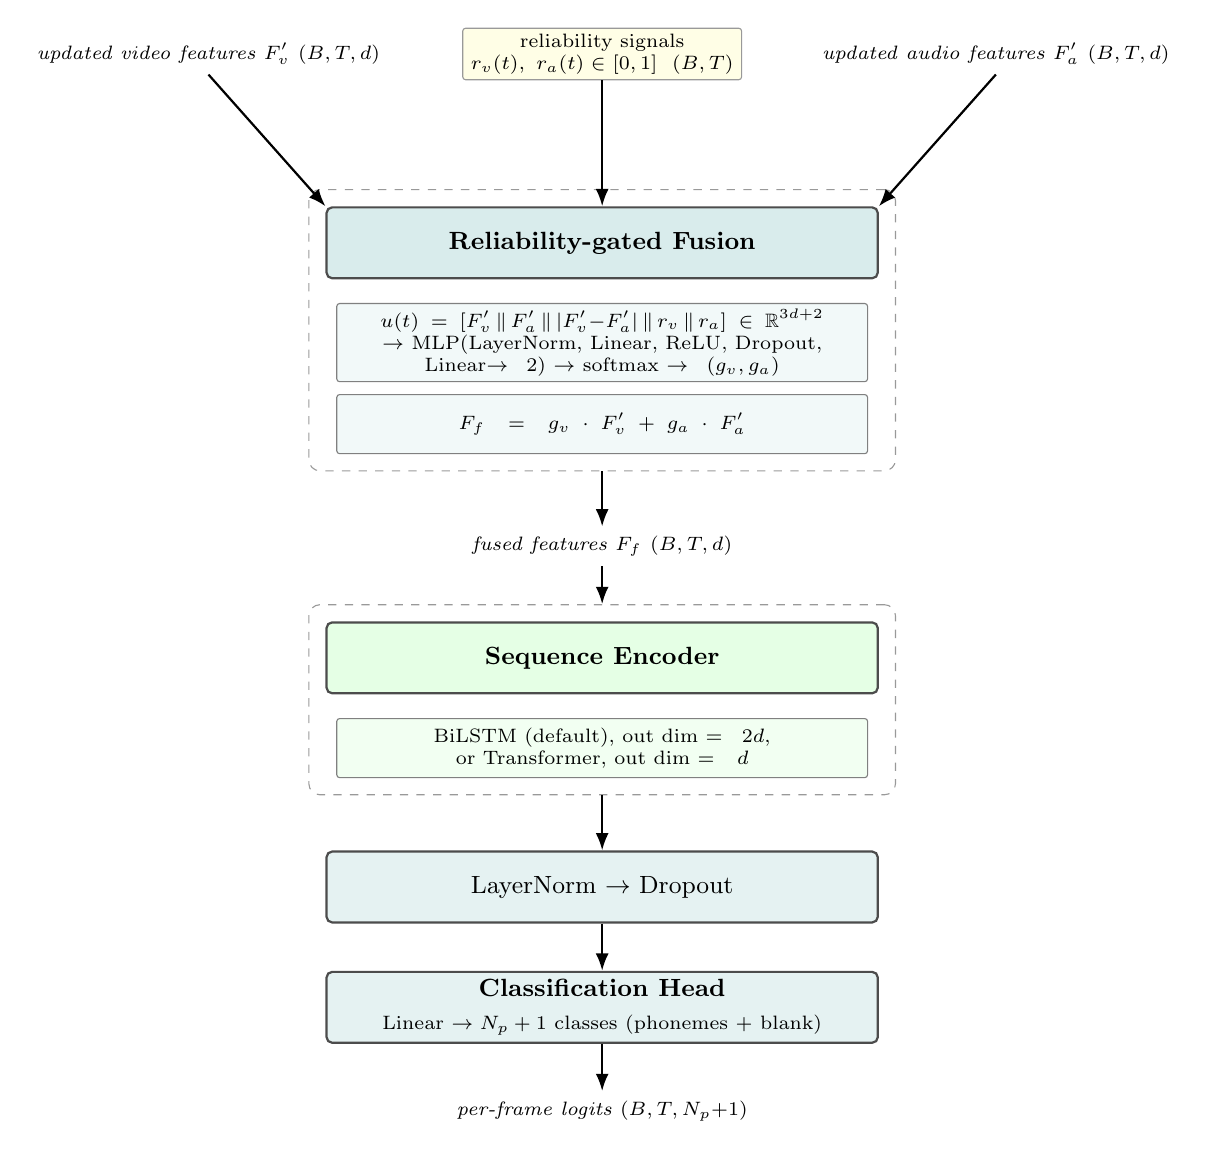
\begin{tikzpicture}[
    font=\small,
    node distance=5mm and 10mm,
    centerblock/.style={
        rectangle, draw=black!70, thick, rounded corners=2pt,
        fill=teal!10, minimum width=70mm, minimum height=9mm,
        align=center, inner sep=2.5pt
    },
    subblock/.style={
        rectangle, draw=black!50, rounded corners=1pt,
        fill=teal!5, minimum width=66mm, minimum height=7.5mm,
        align=center, font=\scriptsize\ttfamily, inner sep=2pt,
        text width=66mm
    },
    iolabel/.style={
        rectangle, draw=none, fill=none, align=center, font=\scriptsize\itshape
    },
    sidelabel/.style={
        rectangle, draw=black!40, fill=yellow!10, rounded corners=1pt,
        align=center, font=\scriptsize, inner sep=2pt
    },
    groupbox/.style={
        rectangle, draw=black!40, dashed, rounded corners=4pt, inner sep=6pt
    },
    arr/.style={-{Latex[length=2.2mm]}, thick},
    every label/.style={font=\scriptsize}
]

% Inputs: updated features from Part I and the reliability signals
\node[iolabel] (v_feat2) at (-50mm,0) {updated video features $F_v'$ $(B,T,d)$};
\node[iolabel] (a_feat2) at (50mm,0) {updated audio features $F_a'$ $(B,T,d)$};
\node[sidelabel, text width=34mm] (rel) at (0,0)
    {reliability signals\\ $r_v(t),\ r_a(t) \in [0,1]$ \ $(B,T)$};

% Reliability-gated fusion
\node[centerblock, below=16mm of rel, fill=teal!15]
    (fusion_title) {\textbf{Reliability-gated Fusion}};
\node[subblock, below=3mm of fusion_title, font=\scriptsize] (fusion_gate)
    {$u(t) = [F_v' \,\Vert\, F_a' \,\Vert\, |F_v'{-}F_a'| \,\Vert\, r_v \,\Vert\, r_a] \in \mathbb{R}^{3d+2}$\\
     $\to$ MLP(LayerNorm, Linear, ReLU, Dropout, Linear$\to2$) $\to$ softmax $\to (g_v, g_a)$};
\node[subblock, below=1.5mm of fusion_gate, font=\scriptsize] (fusion_combine)
    {$F_f = g_v \cdot F_v' + g_a \cdot F_a'$};
\node[groupbox, fit=(fusion_title)(fusion_gate)(fusion_combine)] (fusionbox) {};

% Main encoder pipeline
\node[iolabel, below=7mm of fusionbox] (fused_lbl)
    {fused features $F_f$ $(B,T,d)$};
\node[centerblock, below=7mm of fused_lbl, fill=green!10] (enc_title)
    {\textbf{Sequence Encoder}};
\node[subblock, below=3mm of enc_title, fill=green!5, font=\scriptsize] (bilstm)
    {BiLSTM (default), out dim $=2d$, or Transformer, out dim $=d$};
\node[groupbox, fit=(enc_title)(bilstm)] (encbox) {};
\node[centerblock, below=7mm of encbox] (norm) {LayerNorm $\to$ Dropout};
\node[centerblock, below=6mm of norm] (classifier)
    {\textbf{Classification Head}\\[1pt] \scriptsize Linear $\to N_p+1$ classes (phonemes + blank)};
\node[iolabel, below=6mm of classifier] (logits_lbl) {per-frame logits $(B,T,N_p{+}1)$};

% ------------------------------- Arrows --------------------------------------
\draw[arr] (v_feat2.south) -- (fusion_title.north west);
\draw[arr] (a_feat2.south) -- (fusion_title.north east);
\draw[arr] (rel.south) -- (fusion_title.north);

\draw[arr] (fusionbox.south) -- (fused_lbl.north);
\draw[arr] (fused_lbl.south) -- (encbox.north);
\draw[arr] (encbox.south) -- (norm.north);
\draw[arr] (norm.south) -- (classifier.north);
\draw[arr] (classifier.south) -- (logits_lbl.north);

\end{tikzpicture}
\end{document}
